\scanpage{17}
% Isolated opaque stroke to the left of the date.
\figure{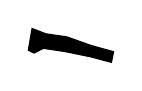
\begin{tikzpicture}[x=1mm,y=1mm]
\fill (0,.4)--(.5,3.3)--(2.3,2.6)--(5,2.2)--(8.1,1.1)--(11,.3)--(10.7,-1.2)--(8.1,-.5)--(4.7,.2)--(2,.6)--(.8,0)--cycle;
\end{tikzpicture}}
\hfill June 15, 1973.\\
Prof Grothendieck,\\

The last proposition stated in the course on alg groups was\unsure{\textsuperscript{-}|\textsuperscript{,}}

``\uline{Prop}: If $k$ is a field, $G$ an affine alg, monoid (resp, an affine alg group).

a) $G=\varprojlim G_i$\qquad where each $G_i$ is an affine alg monoid of finite type over $k$. (resp, affine alg. group of finite type over $k$).

b) If $G$ is of finite type, $\exists$ a closed immersion (of monoids).
\[
G\hookrightarrow.\ \mathrm{GL}(\unsure{n|u})_k\ \unsure{\text{''}|{}^{u}}
\]

I still see difficulty in accepting b). The closed immersion of monoids corresponds to a surjective mapping of coalgebras
\diagram{\begin{minipage}[t]{.39\linewidth}\vspace{0pt}\centering
\begin{tikzcd}[ampersand replacement=\&,column sep=large]
 A \& B\arrow[l,two heads]
\end{tikzcd}
\end{minipage}\hfill
\begin{minipage}[t]{.51\linewidth}\vspace{0pt}
$B$ an algebra representing\\
$\mathrm{GL}(\unsure{n|u})$\par
$A$ an algebra representing\\
$G$,
\end{minipage}}

$B$ has an antipodal map (corresponding to the ``inverse'' map in the on the group object in the cat. $\mathrm{Aff}_k$.)
% archive sheet number: 16
\clearpage
